\chapter{Introducción Específica} % Main chapter title

\label{Chapter2}

%----------------------------------------------------------------------------------------
%	SECTION 1
En este capítulo se detalla la plataforma de hardware utilizada, y se hace una introducción a las herramientas que se tomaron como punto de partida para el desarrollo de este trabajo.
%----------------------------------------------------------------------------------------
\section{La plataforma de Hardware}
\label{sec:plataforma}

La Computadora Industrial Abierta Argentina (CIAA) es un proyecto que comenzó en el año 2013 
gracias a la acción conjunta de \textit{ACSE}\footnote{ACSE: Asociación Civil para la investigación, promoción y desarrollo de los Sistemas electrónicos Embebidos.} y \textit{CADIEEL}\footnote{CADIEEL: Cámara Argentina de Industrias Electrónicas, Electromecánicas y Luminotécnicas.}, dando lugar a una plataforma de hardware que posee dos valiosas características: ser de carácter industrial, es decir, pensada y diseñada para las exigencias de confiabilidad que la industria requiere, y ser abierta bajo licencia BSD, lo cual promueve su uso, modificación y redistribución.

Este trabajo se basó principalmente en la versión educativa de esta computadora, llamada “EDU-CIAA-NXP” cuyo diagrama en bloques se observa en la figura \ref{fig:educiaaBloques}.

\begin{figure}[h]
  \centering
    \includegraphics[width=0.7\textwidth]{Figures/fig_educiaa_diagrama_en_bloques}
  \caption{Diagrama en bloques de la plataforma EDU-CIAA-NXP}
  \label{fig:educiaaBloques}
\end{figure}

La EDU-CIAA-NXP utiliza un microcontrolador NXP LPC 4337 JDB 144 (Dual-core Cortex-M4 + Cortex-M0). Como se observa en la figura \ref{fig:educiaaBloques} la placa tiene 4 pulsadores, 3 leds y un led RGB con los cuales es posible realizar muchos ejercicios, asi como también una conexión USB mediante un chip FT2232 el cual brinda un puerto JTAG y una UART para conectar el microcontrolador con la PC.

La placa también posee dos conectores P1 y P2 de 40 pines cada uno, en donde se encuentran conectados los periféricos del micontrontrolador (GPIOs, UARTs, SPI, I2C, etc.). El diseño fue pensado para proveer una plataforma de desarrollo moderna y económica basada en la CIAA que sirva a docentes y a estudiantes en los cursos de sistemas embebidos y lograr una amplia inserción en el sistema educativo argentino.
En la figura \ref{fig:educiaaPlaca} se muestra una foto de una placa EDU-CIAA-NXP en donde se destaca el detalle de los 4 pulsadores y los leds SMD que permiten realizar ejercicios sin requerir componentes adicionales.

\begin{figure}[h]
  \centering
    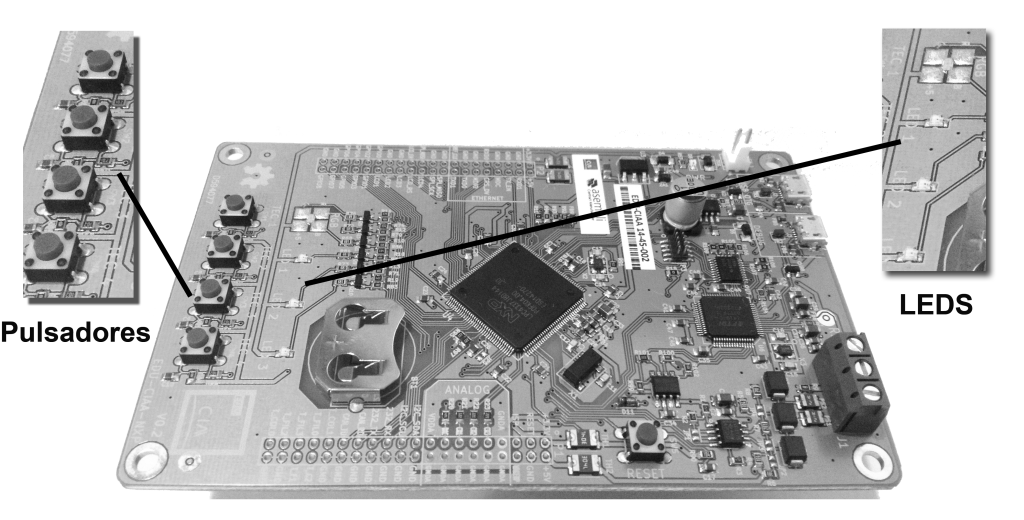
\includegraphics[width=0.7\textwidth]{Figures/fig_educiaa_placa}
  \caption{Foto de una placa EDU-CIAA-NXP}
  \label{fig:educiaaPlaca}
\end{figure}

%----------------------------------------------------------------------------------------

\section{Utilización de MicroPython}
\label{sec:micropython}

El proyecto MicroPython \cite{micropython} es un desarrollo de firmware realizado por Damien George, el cual fue pensado para correr sobre la plataforma Pyboard, desarrollada por Jaltek Systems \cite{jaltek}. Este proyecto permite la ejecución de código Python y la utilización de los periféricos que posee la placa, desde dicho lenguaje.

\begin{figure}[ht]
  \centering
    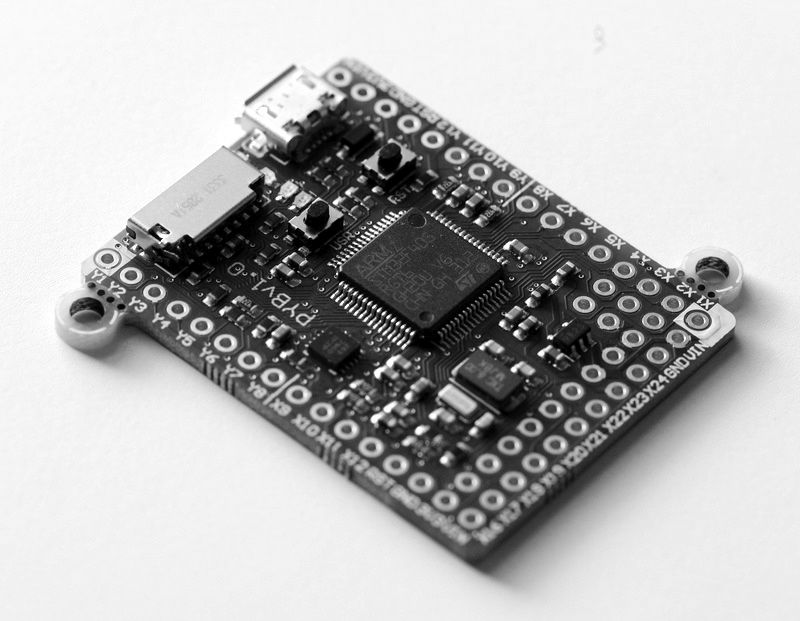
\includegraphics[width=0.4\textwidth]{Figures/fig_pyboard}
  \caption{Foto de una placa Pyboard}
  \label{fig:pyboardPlaca}
\end{figure}

Las características del microcontrolador que posee esta placa, son similares a las de la EDU-CIAA-NXP (Cortex-M4@168Mhz).

%----------------------------------------------------------------------------------------

\section{Firmware: Punto de partida} 

Para obtener la capacidad de ejecutar código Python en la EDU-CIAA-NXP, se adoptó el trabajo de Martin Ribelotta, quien realizó el \textit{port}\footnote{port: Realizar la programación necesaria para que un programa se ejecute en otra plataforma.} del proyecto MicroPython mencionado previamente para esta plataforma \cite{portmicropythonribelotta}.
Este port constaba de la inicialización del intérprete, el cual permitía ejecutar código Python, la inicialización y configuración de la \textit{Garbage Collector}\footnote{Garbage Collector: Gestor automático de memoria dinámica.} y la implementación de un filesystem FAT12 embebido en la memoria de programa del microcontrolador, de manera de poder escribir en forma permanente el código Python en la memoria y luego ser ejecutado desde allí. 

El autor del presente trabajo comenzó a desarrollar el soporte para algunos periféricos a mediados de 2015, ya que el port de Martin Ribelotta no contaba con la implementación para el manejo de dichos periféricos. Esto se tomó como punto de partida y se reescribió y mejoró en gran medida para lograr la calidad del firmware deseada al implementar técnicas de ingeniería de software, verificando su correcto funcionamiento por medio de test unitarios y funcionales los cuales se desarrollan en el capítulo \ref{Chapter4}

Al tomar el port de MicroPython para la EDU-CIAA-NXP desarrollado por Martín Ribelotta, era posible ejecutar un intérprete \textit{REPL}\footnote{REPL: Read Eval Print Loop. Mecanismo que toma una expresión escrita por el usuario, la evalúa y ejecuta, devolviendo el resultado al usuario.} que provee el proyecto, el cual tiene como standard input (stdin) y standard output (stdout) el puerto serie que la placa tiene conectado a través del conversor USB, de modo que en la PC se crea un COM Virtual que permite a cualquier programa que emula una terminal por puerto serial, conectarse a dicho intérprete.

En la figura \ref{fig:conexion} se observan los bloques que modelan la conexión de la placa con la PC. Mediante el circuito integrado FT2232 que posee la placa, se conecta por medio del bus USB, la PC a la EDU-CIAA-NXP, permitiendo visualizar uno de los módulos UART del microcontrolador como un puerto serie en la PC.

\begin{figure}[h]
  \centering
    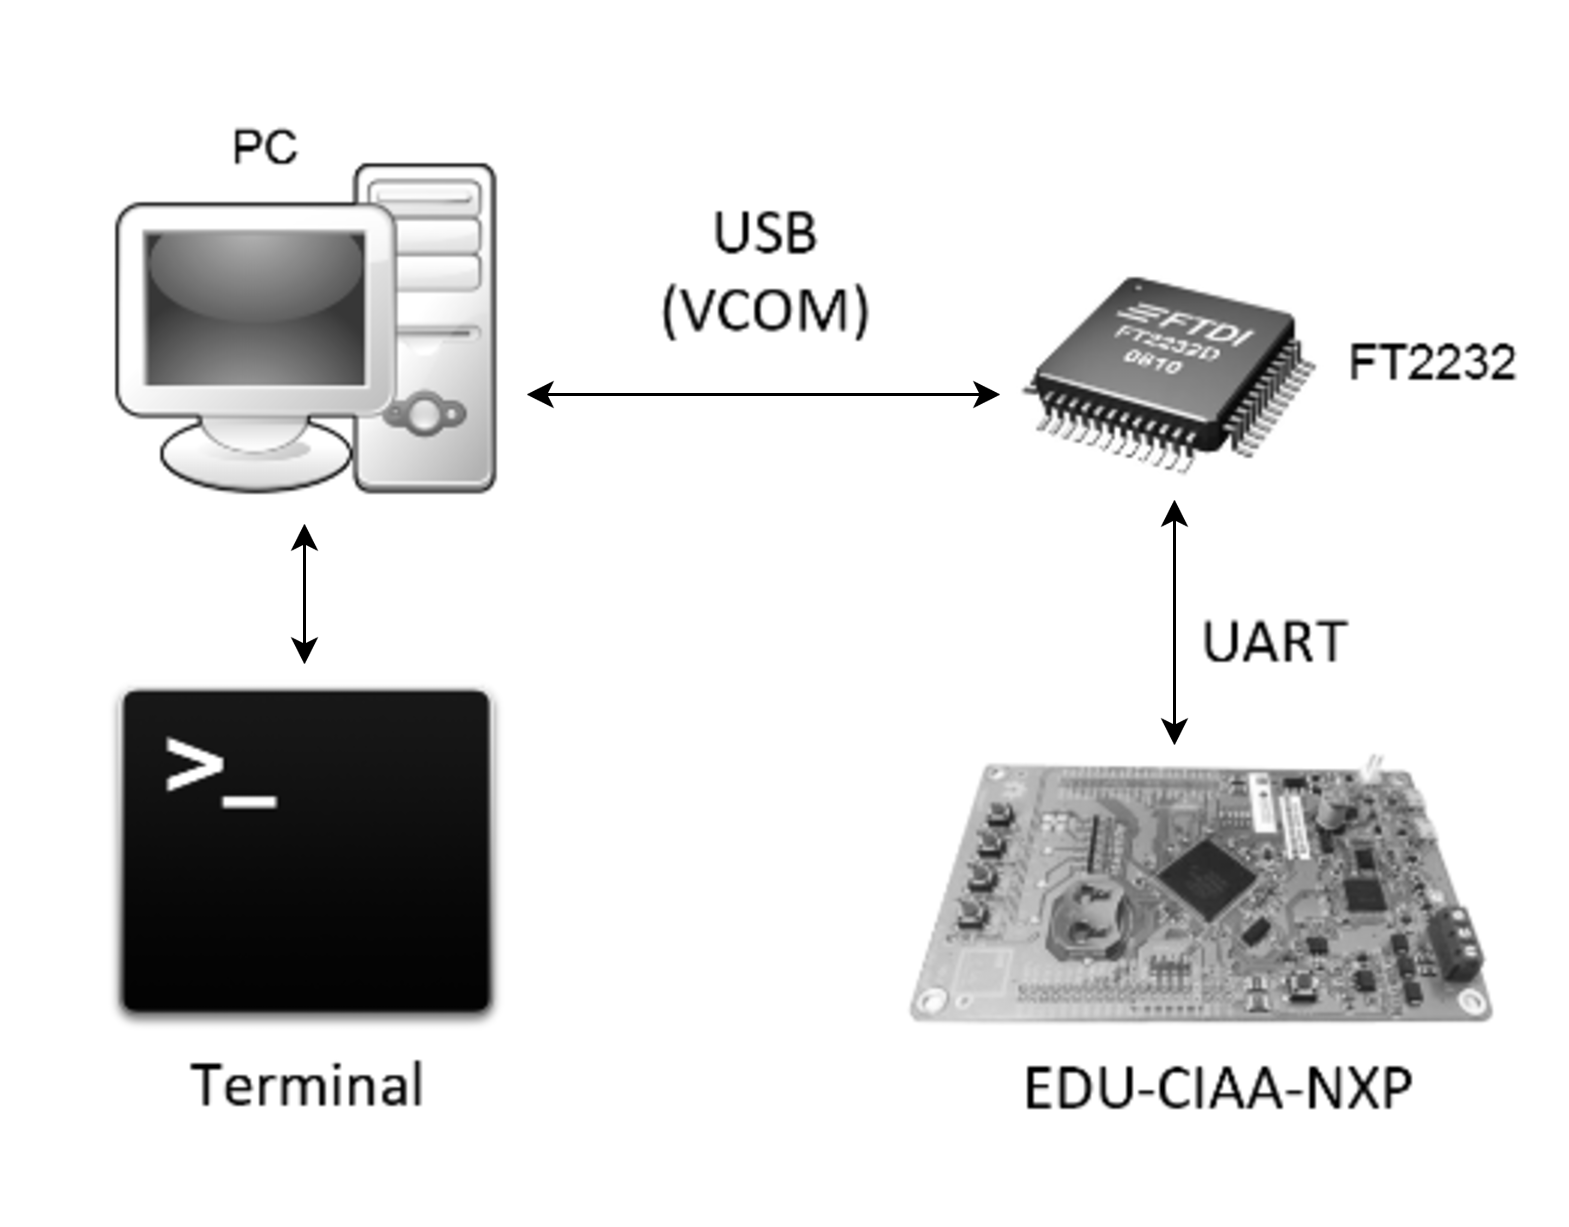
\includegraphics[width=0.6\textwidth]{Figures/fig_conexion}
  \caption{Conexión de la EDU-CIAA-NXP con la PC}
  \label{fig:conexion}
\end{figure}

Esto permite ejecutar programas que no tengan interacción con el resto del hardware, por ejemplo, se puede escribir:

\textbf{{\fontsize{16}{16}\selectfont \textgreater\textgreater}} \texttt{print(“Hola mundo”)}

Una vez ingresado el código, el interprete lo evalúa y ejecuta, y el texto “Hola mundo” se transmite por el stdout, el cual está ligado a la UART conectada al conversor serie-USB, por lo que el texto “Hola mundo” se muestra por la terminal de la PC.

De la misma forma se puede utilizar el sdtin con sentencias como:

\textbf{{\fontsize{16}{16}\selectfont \textgreater\textgreater}} \texttt{n = input(“Ingrese un numero”)}

También se pueden realizar operaciones matemáticas como por ejemplo:

\textbf{{\fontsize{16}{16}\selectfont \textgreater\textgreater}} \texttt{a = 27}\\
\textbf{{\fontsize{16}{16}\selectfont \textgreater\textgreater}} \texttt{b = 3}\\
\textbf{{\fontsize{16}{16}\selectfont \textgreater\textgreater}} \texttt{c = a + b}\\
\textbf{{\fontsize{16}{16}\selectfont \textgreater\textgreater}} \texttt{print(c)}

Este último ejemplo imprime por la terminal el valor 30.

Este port se tomó como punto de partida para incorporar el soporte de los periféricos.

%Pero para interactuar con los periféricos como los pulsadores y los leds, solo existía una versión preliminar de algunas bibliotecas Python creadas previamente por el autor de este trabajo, las cuales se tomaron como punto de partida para el desarrollo profesional de las mismas verificando su correcto funcionamiento por medio de test unitarios y funcionales los cuales se desarrollan en el capítulo \ref{Chapter4}.


%--------------------------------------------------------------------------------------------------------------------------

\section{Software: Punto de partida} 

Para el desarrollo del IDE se tomó como base el proyecto EDILE \cite{edile} el cual se muestra en la figura \ref{fig:edile}. El mismo se encuentra escrito en lenguaje Python y proporciona un procesador de texto con coloreado de palabras clave según el lenguaje seleccionado, el cual se detecta automáticamente por la extensión del archivo que se abre.

\begin{figure}[ht]
  \centering
    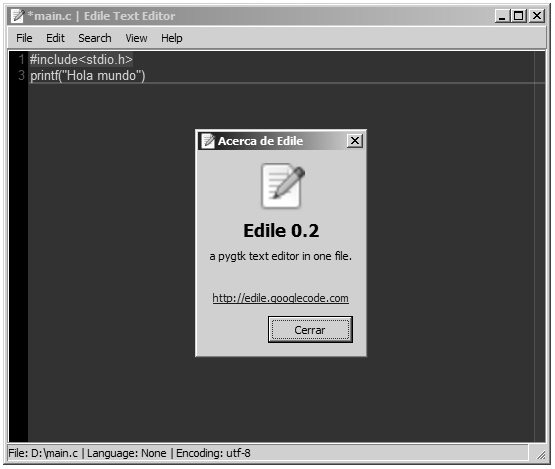
\includegraphics[width=0.7\textwidth]{Figures/fig_edile}
  \caption{Procesador de texto EDILE v0.2}
  \label{fig:edile}
\end{figure}

Debido a que se encuentra programado en Python es muy simple ejecutar el programa en diferentes sistemas operativos, de modo que utilizando este proyecto se cumple con el requerimiento de proveer un software multiplataforma.

Este procesador de texto posee un sistema de plug-ins mediante el cual se simplifica la incorporación de menúes que ejecuten ventanas adicionales que cumplan con cierta funcionalidad, de modo que el diseño de software que se realizó en el presente trabajo fue la incorporación de dichas ventanas y funcionalidades al editor, junto con modificaciones para que solo trabaje con archivos de código Python (.py) y algunas correcciones en el sistema de plug-ins.

Junto con las modificaciones mencionadas, se escribieron test unitarios para las ventanas y clases de lógica desarrolladas, asegurando al igual que en el firmware, la calidad del software requerida para un trabajo de especialización.

%--------------------------------------------------------------------------------------------------------------------------







%----------------------------------------------------------------------------------------


\section{Requerimientos}
\label{sec:req}

En base al estado actual de las herramientas elegidas para el desarrollo del presente trabajo, se enumeran a continuación los requerimientos:

Grupo de requerimientos referidos a las bibliotecas Python:
\begin{enumerate}
	\item  Manejo de los leds que dispone la placa.
	\item  Utilización de los pulsadores.
	\item  Manejo y configuración de los pines designados como GPIO. 
	\item  Configuración y utilización de la UART.
	\item  Configuración y utilización de la interface RS485.
	\item  Lectura de las entradas ADC.
	\item  Salida DAC.
	\item  Utilización de la EEPROM interna.
	\item  Utilización de Timers.
\end{enumerate}

Grupo de requerimientos referidos al entorno de desarrollo:
\begin{enumerate}
	\item  El software deberá ser multiplataforma (Windows/Linux/OSX).
	\item  No debe ser necesario recompilar el firmware de la placa para cambiar el código de python.
	\item  El programa de python se enviará por el COM virtual generado al conectar la placa a la PC. 
	\item  El software deberá tener embebida una terminal serial, por donde se implementará la interfaz de salida y entrada estándar del programa de Python. 
	\item  El software deberá tener porciones de código de ejemplo que puedan insertarse fácilmente junto con lo que el usuario programa (Snippets)
	\item  El software deberá tener links para acceder fácilmente a la documentación online y a los proyectos de ejemplo.
\end{enumerate}

Grupo de requerimientos referidos a los proyectos de ejemplo:
\begin{enumerate}
	\item  Los proyectos de ejemplo serán divididos en tres categorías: Inicial, Intermedio y Avanzado. 
	\item  Los proyectos de ejemplo consistirán en el código fuente, la explicación del mismo en forma detallada, y un esquemático de conexión con componentes externos en el caso que se requiera.
	\item  Los proyectos de ejemplo están basados en los proyectos típicos de electrónica que se realizan en escuelas secundarias. 
\end{enumerate}

Grupo de requerimientos generales:
\begin{enumerate}
	\item  El acceso a la información del proyecto será libre y gratuita.  
	\item  Se publicará la documentación de las bibliotecas de Python disponibles para programar.
\end{enumerate}


%----------------------------------------------------------------------------------------


